\documentclass{llncs}\usepackage[]{graphicx}\usepackage[]{color}
%% maxwidth is the original width if it is less than linewidth
%% otherwise use linewidth (to make sure the graphics do not exceed the margin)
\makeatletter
\def\maxwidth{ %
  \ifdim\Gin@nat@width>\linewidth
    \linewidth
  \else
    \Gin@nat@width
  \fi
}
\makeatother

\definecolor{fgcolor}{rgb}{0.345, 0.345, 0.345}
\newcommand{\hlnum}[1]{\textcolor[rgb]{0.686,0.059,0.569}{#1}}%
\newcommand{\hlstr}[1]{\textcolor[rgb]{0.192,0.494,0.8}{#1}}%
\newcommand{\hlcom}[1]{\textcolor[rgb]{0.678,0.584,0.686}{\textit{#1}}}%
\newcommand{\hlopt}[1]{\textcolor[rgb]{0,0,0}{#1}}%
\newcommand{\hlstd}[1]{\textcolor[rgb]{0.345,0.345,0.345}{#1}}%
\newcommand{\hlkwa}[1]{\textcolor[rgb]{0.161,0.373,0.58}{\textbf{#1}}}%
\newcommand{\hlkwb}[1]{\textcolor[rgb]{0.69,0.353,0.396}{#1}}%
\newcommand{\hlkwc}[1]{\textcolor[rgb]{0.333,0.667,0.333}{#1}}%
\newcommand{\hlkwd}[1]{\textcolor[rgb]{0.737,0.353,0.396}{\textbf{#1}}}%

\usepackage{framed}
\makeatletter
\newenvironment{kframe}{%
 \def\at@end@of@kframe{}%
 \ifinner\ifhmode%
  \def\at@end@of@kframe{\end{minipage}}%
  \begin{minipage}{\columnwidth}%
 \fi\fi%
 \def\FrameCommand##1{\hskip\@totalleftmargin \hskip-\fboxsep
 \colorbox{shadecolor}{##1}\hskip-\fboxsep
     % There is no \\@totalrightmargin, so:
     \hskip-\linewidth \hskip-\@totalleftmargin \hskip\columnwidth}%
 \MakeFramed {\advance\hsize-\width
   \@totalleftmargin\z@ \linewidth\hsize
   \@setminipage}}%
 {\par\unskip\endMakeFramed%
 \at@end@of@kframe}
\makeatother

\definecolor{shadecolor}{rgb}{.97, .97, .97}
\definecolor{messagecolor}{rgb}{0, 0, 0}
\definecolor{warningcolor}{rgb}{1, 0, 1}
\definecolor{errorcolor}{rgb}{1, 0, 0}
\newenvironment{knitrout}{}{} % an empty environment to be redefined in TeX

\usepackage{alltt}
\usepackage{listings}
\usepackage{moreverb}
\usepackage{inconsolata}
\pagestyle{plain}


\IfFileExists{upquote.sty}{\usepackage{upquote}}{}
\begin{document}

\title{Problem Set 4}
\author{Thibault Doutre, ID : 26980469}
\institute{STAT 243 : Introduction to Statistical Computing}
\date{}
\maketitle
\bigbreak
\noindent
I worked on my own.
%%%%%%%%%%%%%%%%%%%%%%%%%%%%%%%%%%%%%%%%%%%%%%%%%%%%%%%%%%%
\section{Problem 1}
%%%%%%%%%%%%%%%%%%%%%%%%%%%%%%%%%%%%%%%%%%%%%%%%%%%%%%%%%%%%
\subsection{Question a}
The problem comes from the difference between global and local variables. 
\begin{knitrout}
\definecolor{shadecolor}{rgb}{0.969, 0.969, 0.969}\color{fgcolor}\begin{kframe}
\begin{alltt}
\hlkwd{set.seed}\hlstd{(}\hlnum{0}\hlstd{)}
\hlkwd{runif}\hlstd{(}\hlnum{1}\hlstd{)}
\end{alltt}
\begin{lstlisting}[basicstyle=\ttfamily,breaklines=true]
## [1] 0.8966972
\end{lstlisting}
\begin{alltt}
\hlcom{# save the seed into a file}
\hlkwd{save}\hlstd{(.Random.seed,} \hlkwc{file} \hlstd{=} \hlstr{'tmp.Rda'}\hlstd{)}
\hlcom{# result}
\hlkwd{runif}\hlstd{(}\hlnum{1}\hlstd{)}
\end{alltt}
\begin{lstlisting}[basicstyle=\ttfamily,breaklines=true]
## [1] 0.2655087
\end{lstlisting}
\begin{alltt}
\hlkwd{load}\hlstd{(}\hlstr{'tmp.Rda'}\hlstd{)}
\hlcom{#same result than before}
\hlkwd{runif}\hlstd{(}\hlnum{1}\hlstd{)}
\end{alltt}
\begin{lstlisting}[basicstyle=\ttfamily,breaklines=true]
## [1] 0.2655087
\end{lstlisting}
\end{kframe}
\end{knitrout}
\noindent
Now, we debug the code by printing out the assertion of the equality between the random seed immediately after having loaded the file and the random seed of the global environment. And we see that it is false.
\begin{knitrout}
\definecolor{shadecolor}{rgb}{0.969, 0.969, 0.969}\color{fgcolor}\begin{kframe}
\begin{alltt}
\hlcom{# Debug}
\hlstd{tmp} \hlkwb{<-} \hlkwa{function}\hlstd{() \{}
  \hlkwd{load}\hlstd{(}\hlstr{'tmp.Rda'}\hlstd{)}
  \hlkwd{print}\hlstd{(}\hlkwd{identical}\hlstd{(.Random.seed,.GlobalEnv}\hlopt{$}\hlstd{.Random.seed))}
  \hlkwd{runif}\hlstd{(}\hlnum{1}\hlstd{)}
\hlstd{\}}
\hlkwd{tmp}\hlstd{()}
\end{alltt}
\begin{lstlisting}[basicstyle=\ttfamily,breaklines=true]
## [1] FALSE
\end{lstlisting}
\begin{lstlisting}[basicstyle=\ttfamily,breaklines=true]
## [1] 0.3721239
\end{lstlisting}
\end{kframe}
\end{knitrout}
\noindent
To correct the code, I load the random seed in the global environment.
\begin{knitrout}
\definecolor{shadecolor}{rgb}{0.969, 0.969, 0.969}\color{fgcolor}\begin{kframe}
\begin{alltt}
\hlstd{tmp} \hlkwb{<-} \hlkwa{function}\hlstd{() \{}
  \hlkwd{load}\hlstd{(}\hlstr{'tmp.Rda'}\hlstd{,}\hlkwc{envir} \hlstd{=} \hlkwd{globalenv}\hlstd{())}
  \hlkwd{runif}\hlstd{(}\hlnum{1}\hlstd{)}
\hlstd{\}}
\hlcom{# Expected result}
\hlkwd{tmp}\hlstd{()}
\end{alltt}
\begin{lstlisting}[basicstyle=\ttfamily,breaklines=true]
## [1] 0.2655087
\end{lstlisting}
\end{kframe}
\end{knitrout}



%%%%%%%%%%%%%%%%%%%%%%%%%%%%%%%%%%%%%%%%%%%%%%%%%%%%%%%%%%%
\section{Problem 2}
%%%%%%%%%%%%%%%%%%%%%%%%%%%%%%%%%%%%%%%%%%%%%%%%%%%%%%%%%%%%
First, set the libraries, the global variables and the wd.
\begin{knitrout}
\definecolor{shadecolor}{rgb}{0.969, 0.969, 0.969}\color{fgcolor}\begin{kframe}
\begin{alltt}
\hlkwd{setwd}\hlstd{(}\hlstr{"/Users/doutre/Documents/stat243/ps4"}\hlstd{)}
\hlkwd{library}\hlstd{(fields)}
\end{alltt}


{\ttfamily\noindent\itshape\color{messagecolor}{\#\# Loading required package: spam\\\#\# Loading required package: grid\\\#\# Spam version 1.0-1 (2014-09-09) is loaded.\\\#\# Type 'help( Spam)' or 'demo( spam)' for a short introduction \\\#\# and overview of this package.\\\#\# Help for individual functions is also obtained by adding the\\\#\# suffix '.spam' to the function name, e.g. 'help( chol.spam)'.\\\#\# \\\#\# Attaching package: 'spam'\\\#\# \\\#\# The following objects are masked from 'package:base':\\\#\# \\\#\#\ \ \ \  backsolve, forwardsolve\\\#\# \\\#\# Loading required package: maps\\\#\# \\\#\# Attaching package: 'fields'\\\#\# \\\#\# The following object is masked from 'package:maps':\\\#\# \\\#\#\ \ \ \  ozone}}\begin{alltt}
\hlkwd{library}\hlstd{(rbenchmark)}

\hlcom{## Global variables}
\hlstd{p} \hlkwb{=} \hlnum{0.3}
\hlstd{φ} \hlkwb{=} \hlnum{0.5}
\end{alltt}
\end{kframe}
\end{knitrout}
\subsection{Question a}
In order to compute the sum, I first create the function f(k,n,p,phi) and then apply it for all k in an other function, using lapply. We have to do the computations in the log scale because R cannot handle operations on too large numbers. Therefore, it is more appropriate to take the exponential of the log of the product of terms in the expression of f(k,n,p,phi).
\begin{knitrout}
\definecolor{shadecolor}{rgb}{0.969, 0.969, 0.969}\color{fgcolor}\begin{kframe}
\begin{alltt}
\hlstd{log_f} \hlkwb{=} \hlkwa{function}\hlstd{(}\hlkwc{k}\hlstd{,}\hlkwc{n}\hlstd{,}\hlkwc{p}\hlstd{,}\hlkwc{φ}\hlstd{)\{}
  \hlkwa{if} \hlstd{(k}\hlopt{==}\hlnum{0} \hlopt{||} \hlstd{k}\hlopt{==}\hlstd{n)}
    \hlkwd{return}\hlstd{((n}\hlopt{-}\hlstd{k)}\hlopt{*}\hlstd{φ}\hlopt{*}\hlkwd{log}\hlstd{(}\hlnum{1}\hlopt{-}\hlstd{p)}\hlopt{+} \hlstd{k}\hlopt{*}\hlstd{φ}\hlopt{*}\hlkwd{log}\hlstd{(p) )}
  \hlkwa{else}
    \hlkwd{return}\hlstd{(}\hlkwd{lchoose}\hlstd{(n,k)}\hlopt{+}
             \hlstd{(}\hlnum{1}\hlopt{-}\hlstd{φ)}\hlopt{*}\hlstd{(k}\hlopt{*}\hlkwd{log}\hlstd{(k)} \hlopt{+} \hlstd{(n}\hlopt{-}\hlstd{k)}\hlopt{*}\hlkwd{log}\hlstd{(n}\hlopt{-}\hlstd{k)} \hlopt{-} \hlstd{n}\hlopt{*}\hlkwd{log}\hlstd{(n))}\hlopt{+}
            \hlstd{φ}\hlopt{*}\hlstd{(k}\hlopt{*}\hlkwd{log}\hlstd{(p)} \hlopt{+} \hlstd{(n}\hlopt{-}\hlstd{k)}\hlopt{*}\hlkwd{log}\hlstd{(}\hlnum{1}\hlopt{-}\hlstd{p)))}
\hlstd{\}}

\hlcom{# using lapply}
\hlstd{sum_f} \hlkwb{=} \hlkwa{function}\hlstd{(}\hlkwc{n}\hlstd{,}\hlkwc{p}\hlstd{,}\hlkwc{φ}\hlstd{)\{}
  \hlstd{l} \hlkwb{=} \hlkwd{as.list}\hlstd{(}\hlnum{0}\hlopt{:}\hlstd{n)}
  \hlstd{fk} \hlkwb{=} \hlkwd{lapply}\hlstd{(l,}\hlkwa{function}\hlstd{(}\hlkwc{k}\hlstd{)} \hlkwd{exp}\hlstd{(}\hlkwd{log_f}\hlstd{(k,n,p,φ)))}
  \hlkwd{return}\hlstd{(}\hlkwd{Reduce}\hlstd{(}\hlstr{"+"}\hlstd{,fk))}
\hlstd{\}}
\hlcom{# Example}
\hlkwd{sum_f}\hlstd{(}\hlnum{200}\hlstd{,p,φ)}
\end{alltt}
\begin{lstlisting}[basicstyle=\ttfamily,breaklines=true]
## [1] 1.416484
\end{lstlisting}
\end{kframe}
\end{knitrout}
\subsection{Question b}
Now, I do the calsulation in the vectorized way. The code is a bit messy because it is optimized. But basically, here are the tips:
\begin{itemize}
\item Write the formula in the most factorized way
\item Do not do twice the same computation, instead store it into a variable
\item lgamma is better than lfactorial or lchoose
\item crossprod is very efficient for summing a vector
\end{itemize}
It is important to notice that the cases k=0 and k=n are added at the last moment and the vectors used before are of length n-1.
\begin{knitrout}
\definecolor{shadecolor}{rgb}{0.969, 0.969, 0.969}\color{fgcolor}\begin{kframe}
\begin{alltt}
\hlstd{sum_f_vect} \hlkwb{=} \hlkwa{function}\hlstd{(}\hlkwc{n}\hlstd{,}\hlkwc{p}\hlstd{,}\hlkwc{φ}\hlstd{)\{}
  \hlstd{ones}\hlkwb{=}\hlkwd{matrix}\hlstd{(}\hlnum{1}\hlstd{,}\hlkwc{nrow}\hlstd{=n}\hlopt{-}\hlnum{1}\hlstd{,}\hlkwc{ncol}\hlstd{=}\hlnum{1}\hlstd{)}
  \hlstd{v}\hlkwb{=}\hlnum{1}\hlopt{:}\hlstd{(n}\hlopt{-}\hlnum{1}\hlstd{)}
  \hlstd{n_v}\hlkwb{=} \hlopt{-}\hlstd{v}
  \hlstd{n_and_n_v}\hlkwb{=}\hlstd{(n}\hlopt{+}\hlstd{n_v)}
  \hlstd{phi_phiBis}\hlkwb{=}\hlkwd{exp}\hlstd{(}\hlopt{-}\hlkwd{log}\hlstd{(}\hlnum{1}\hlopt{/}\hlstd{φ}\hlopt{-}\hlnum{1}\hlstd{))}
  \hlstd{s_bounds} \hlkwb{=} \hlkwd{exp}\hlstd{((}\hlkwd{lgamma}\hlstd{(n}\hlopt{+}\hlnum{1}\hlstd{)}\hlopt{-}\hlstd{(}\hlkwd{lgamma}\hlstd{(v}\hlopt{+}\hlnum{1}\hlstd{)}\hlopt{+}\hlkwd{lgamma}\hlstd{(n}\hlopt{+}\hlstd{n_v}\hlopt{+}\hlnum{1}\hlstd{)))}\hlopt{+}
                   \hlstd{(}\hlnum{1}\hlopt{-}\hlstd{φ)}\hlopt{*}\hlstd{(v}\hlopt{*}\hlstd{(}\hlkwd{log}\hlstd{(v)}\hlopt{+}\hlkwd{log}\hlstd{(p)}\hlopt{*}\hlstd{phi_phiBis)} \hlopt{+}
                   \hlstd{n_and_n_v}\hlopt{*}\hlstd{(}\hlkwd{log}\hlstd{(n_and_n_v)}\hlopt{+}\hlstd{phi_phiBis}\hlopt{*}\hlkwd{log}\hlstd{(}\hlnum{1}\hlopt{-}\hlstd{p))} \hlopt{-}
                   \hlstd{n}\hlopt{*}\hlkwd{log}\hlstd{(n)))}
  \hlkwd{return}\hlstd{(} \hlkwd{exp}\hlstd{((n}\hlopt{*}\hlstd{φ)}\hlopt{*}\hlkwd{log}\hlstd{((}\hlnum{1}\hlopt{-}\hlstd{p)}\hlopt{*}\hlstd{p))}\hlopt{+}\hlkwd{crossprod}\hlstd{(s_bounds,ones))}
\hlstd{\}}
\hlcom{# Example}
\hlkwd{sum_f}\hlstd{(}\hlnum{200}\hlstd{,p,φ)}
\end{alltt}
\begin{lstlisting}[basicstyle=\ttfamily,breaklines=true]
## [1] 1.416484
\end{lstlisting}
\end{kframe}
\end{knitrout}
\noindent
Here is the performances:
\begin{knitrout}
\definecolor{shadecolor}{rgb}{0.969, 0.969, 0.969}\color{fgcolor}\begin{kframe}
\begin{alltt}
\hlkwd{Rprof}\hlstd{(}\hlstr{"sum_f.txt"}\hlstd{,}\hlkwc{interval} \hlstd{=} \hlnum{1e-5}\hlstd{)}
\hlstd{out}\hlkwb{=}\hlkwd{sum_f_vect}\hlstd{(}\hlnum{1e7}\hlstd{,p,φ)}
\hlkwd{Rprof}\hlstd{(}\hlkwa{NULL}\hlstd{)}
\hlkwd{summaryRprof}\hlstd{(}\hlstr{"sum_f.txt"}\hlstd{)}\hlopt{$}\hlstd{by.self}
\end{alltt}
\begin{lstlisting}[basicstyle=\ttfamily,breaklines=true]
##              self.time self.pct total.time total.pct
## "+"              0.153    42.78      0.153     42.78
## "matrix"         0.111    31.07      0.111     31.07
## "sum_f_vect"     0.055    15.42      0.358     99.98
## ":"              0.019     5.31      0.019      5.31
## "-"              0.017     4.73      0.017      4.73
## "lgamma"         0.002     0.58      0.002      0.58
\end{lstlisting}
\begin{alltt}
\hlkwd{benchmark}\hlstd{(}
  \hlkwc{out} \hlstd{=} \hlkwd{sum_f}\hlstd{(}\hlnum{200}\hlstd{,p,φ) ,}
  \hlkwc{out_vect} \hlstd{=} \hlkwd{sum_f_vect}\hlstd{(}\hlnum{200}\hlstd{,p,φ),}
  \hlkwc{replications} \hlstd{=} \hlnum{1000}\hlstd{,}
  \hlkwc{columns}\hlstd{=}\hlkwd{c}\hlstd{(}\hlstr{'test'}\hlstd{,} \hlstr{'elapsed'}\hlstd{,} \hlstr{'replications'}\hlstd{))}
\end{alltt}
\begin{lstlisting}[basicstyle=\ttfamily,breaklines=true]
##       test elapsed replications
## 1      out   1.060         1000
## 2 out_vect   0.052         1000
\end{lstlisting}
\end{kframe}
\end{knitrout}
\noindent
We can see that the vectorized way is 100 times more efficient than the naive approach.


%%%%%%%%%%%%%%%%%%%%%%%%%%%%%%%%%%%%%%%%%%%%%%%%%%%%%%%%%%%
\section{Problem 3}
%%%%%%%%%%%%%%%%%%%%%%%%%%%%%%%%%%%%%%%%%%%%%%%%%%%%%%%%%%%%
\noindent
First of all, let's set the wd, load some libraries and the data provided. I also set a global variable, n, which is the length of IDsA or IDsB (they are equal).
\begin{knitrout}
\definecolor{shadecolor}{rgb}{0.969, 0.969, 0.969}\color{fgcolor}\begin{kframe}
\begin{alltt}
\hlkwd{setwd}\hlstd{(}\hlstr{"/Users/doutre/Documents/stat243/ps4"}\hlstd{)}
\hlkwd{load}\hlstd{(}\hlstr{"./mixedMember.Rda"}\hlstd{)}
\hlkwd{library}\hlstd{(rbenchmark)}
\hlkwd{library}\hlstd{(fields)}
\hlkwd{library}\hlstd{(plyr)}
\end{alltt}


{\ttfamily\noindent\itshape\color{messagecolor}{\#\# \\\#\# Attaching package: 'plyr'\\\#\# \\\#\# The following object is masked from 'package:fields':\\\#\# \\\#\#\ \ \ \  ozone\\\#\# \\\#\# The following object is masked from 'package:maps':\\\#\# \\\#\#\ \ \ \  ozone}}\begin{alltt}
\hlkwd{library}\hlstd{(Matrix)}
\hlkwd{library}\hlstd{(microbenchmark)}

\hlcom{## Global variables}
\hlstd{n}\hlkwb{=}\hlkwd{length}\hlstd{(IDsA)} \hlcom{#IDsB has the same length}
\end{alltt}
\end{kframe}
\end{knitrout}

\subsection{Question a}
In one line, I compute the sum for cases A and B, and do a benchmark to see the average speed on 10 replications.
\begin{knitrout}
\definecolor{shadecolor}{rgb}{0.969, 0.969, 0.969}\color{fgcolor}\begin{kframe}
\begin{alltt}
\hlcom{# For A}
\hlstd{outA} \hlkwb{=} \hlkwd{sapply}\hlstd{(}\hlnum{1}\hlopt{:}\hlstd{n,}\hlkwa{function}\hlstd{(}\hlkwc{i}\hlstd{)} \hlkwd{sum}\hlstd{(wgtsA[[i]]}\hlopt{*}\hlstd{muA[IDsA[[i]]]))}
\hlcom{# For B}
\hlstd{outB} \hlkwb{=} \hlkwd{sapply}\hlstd{(}\hlnum{1}\hlopt{:}\hlstd{n,}\hlkwa{function}\hlstd{(}\hlkwc{i}\hlstd{)} \hlkwd{sum}\hlstd{(wgtsB[[i]]}\hlopt{*}\hlstd{muB[IDsB[[i]]]))}

\hlcom{# speed calculation}
\hlkwd{benchmark}\hlstd{(}
  \hlkwc{outA}\hlstd{=}\hlkwd{sapply}\hlstd{(}\hlnum{1}\hlopt{:}\hlstd{n,}\hlkwa{function}\hlstd{(}\hlkwc{i}\hlstd{)} \hlkwd{sum}\hlstd{(wgtsA[[i]]}\hlopt{*}\hlstd{muA[IDsA[[i]]])),}
  \hlkwc{outB}\hlstd{=}\hlkwd{sapply}\hlstd{(}\hlnum{1}\hlopt{:}\hlstd{n,}\hlkwa{function}\hlstd{(}\hlkwc{i}\hlstd{)} \hlkwd{sum}\hlstd{(wgtsB[[i]]}\hlopt{*}\hlstd{muB[IDsB[[i]]])),}
  \hlkwc{replications} \hlstd{=} \hlnum{10}\hlstd{,}
  \hlkwc{columns}\hlstd{=}\hlkwd{c}\hlstd{(}\hlstr{'test'}\hlstd{,} \hlstr{'elapsed'}\hlstd{,} \hlstr{'replications'}\hlstd{))}
\end{alltt}
\begin{lstlisting}[basicstyle=\ttfamily,breaklines=true]
##   test elapsed replications
## 1 outA   1.635           10
## 2 outB   1.710           10
\end{lstlisting}
\end{kframe}
\end{knitrout}

\subsection{Question b and c}
The basic idea of what I have implemented is based on the trace of a product of matrices. Indeed, we can easily see that the sum is the trace of the matrix product of MU and W, with MU and W well defined. Seeing things this way, it is really fast to compute the sums which are the sums over the lines of MU*W (* is the Hilbert product for matrices, just like in R). \\
But is is important to notice that MU depends on mu, and that it is unfortunate since we want to transform the data, setting aside mu. \\
So, this is how I proceed:
\begin {itemize}
\item Transform IDs data so each colum indicates the index of mu. In other words each column has ones at the indices of IDs.
\begin{knitrout}
\definecolor{shadecolor}{rgb}{0.969, 0.969, 0.969}\color{fgcolor}\begin{kframe}
\begin{alltt}
\hlcom{# Transform function : add zeros in the middle}
\hlstd{transform_ID} \hlkwb{=} \hlkwa{function}\hlstd{(}\hlkwc{l}\hlstd{,}\hlkwc{max.len}\hlstd{)\{}
  \hlstd{M}\hlkwb{=}\hlkwd{matrix}\hlstd{(}\hlkwd{rep}\hlstd{(}\hlnum{0}\hlstd{,max.len}\hlopt{*}\hlkwd{length}\hlstd{(l)),}\hlkwc{nrow}\hlstd{=max.len)}
  \hlkwa{for} \hlstd{(i} \hlkwa{in} \hlnum{1}\hlopt{:}\hlkwd{length}\hlstd{(l))\{}
    \hlstd{li}\hlkwb{=}\hlstd{l[[i]]}
    \hlstd{M[li,i]}\hlkwb{=}\hlnum{1}
  \hlstd{\}}
  \hlkwd{return}\hlstd{(M)}
\hlstd{\}}
\hlcom{# Example}
\hlkwd{transform_ID}\hlstd{(IDsB,}\hlkwd{length}\hlstd{(muB))[,}\hlnum{1}\hlopt{:}\hlnum{3}\hlstd{]}
\end{alltt}
\begin{lstlisting}[basicstyle=\ttfamily,breaklines=true]
##       [,1] [,2] [,3]
##  [1,]    0    0    0
##  [2,]    1    0    0
##  [3,]    1    1    1
##  [4,]    1    1    1
##  [5,]    1    0    0
##  [6,]    1    0    0
##  [7,]    1    0    0
##  [8,]    1    0    1
##  [9,]    1    0    1
## [10,]    1    1    0
\end{lstlisting}
\begin{alltt}
\hlcom{# Original data}
\hlkwd{head}\hlstd{(IDsB,}\hlnum{3}\hlstd{)}
\end{alltt}
\begin{lstlisting}[basicstyle=\ttfamily,breaklines=true]
## [[1]]
## [1]  2  7  6  3  4  5  9  8 10
## 
## [[2]]
## [1] 10  3  4
## 
## [[3]]
## [1] 3 9 4 8
\end{lstlisting}
\end{kframe}
\end{knitrout}
\item Transform the matrix of weigths such that the size of the matrix is the same as the transformed IDs and each ones in this latter is filled with corresponding weights values.
\begin{knitrout}
\definecolor{shadecolor}{rgb}{0.969, 0.969, 0.969}\color{fgcolor}\begin{kframe}
\begin{alltt}
\hlcom{# Transform W }
\hlstd{transform_W} \hlkwb{=} \hlkwa{function}\hlstd{(}\hlkwc{l}\hlstd{,}\hlkwc{ID_transformed}\hlstd{)\{}
  \hlstd{M}\hlkwb{=}\hlstd{ID_transformed}
  \hlkwa{for} \hlstd{(i} \hlkwa{in} \hlnum{1}\hlopt{:}\hlkwd{length}\hlstd{(l))\{}
    \hlstd{li}\hlkwb{=}\hlstd{l[[i]]}
    \hlstd{M[,i][M[,i]} \hlopt{!=} \hlnum{0}\hlstd{]}\hlkwb{=}\hlstd{li}
  \hlstd{\}}
  \hlkwd{return}\hlstd{(M)}
\hlstd{\}}
\hlcom{# Example}
\hlkwd{transform_W}\hlstd{(wgtsB,}\hlkwd{transform_ID}\hlstd{(IDsB,}\hlkwd{length}\hlstd{(muB)))[,}\hlnum{1}\hlopt{:}\hlnum{3}\hlstd{]}
\end{alltt}
\begin{lstlisting}[basicstyle=\ttfamily,breaklines=true]
##              [,1]       [,2]      [,3]
##  [1,] 0.000000000 0.00000000 0.0000000
##  [2,] 0.226200194 0.00000000 0.0000000
##  [3,] 0.469188914 0.81031321 0.2653353
##  [4,] 0.011783225 0.15188043 0.3655552
##  [5,] 0.058049207 0.00000000 0.0000000
##  [6,] 0.078030098 0.00000000 0.0000000
##  [7,] 0.005137179 0.00000000 0.0000000
##  [8,] 0.049490784 0.00000000 0.1903563
##  [9,] 0.018964598 0.00000000 0.1787532
## [10,] 0.083155801 0.03780636 0.0000000
\end{lstlisting}
\begin{alltt}
\hlcom{# Original data}
\hlkwd{head}\hlstd{(wgtsB,}\hlnum{3}\hlstd{)}
\end{alltt}
\begin{lstlisting}[basicstyle=\ttfamily,breaklines=true]
## [[1]]
## [1] 0.226200194 0.469188914 0.011783225 0.058049207
## [5] 0.078030098 0.005137179 0.049490784 0.018964598
## [9] 0.083155801
## 
## [[2]]
## [1] 0.81031321 0.15188043 0.03780636
## 
## [[3]]
## [1] 0.2653353 0.3655552 0.1903563 0.1787532
\end{lstlisting}
\end{kframe}
\end{knitrout}
\item Now, we may be tempted to compute the Trace of the product of matrices issued from these two functions. But when the IDs are mapped in a special way, so we would have to correctly assign the mus to the IDs functions. But we do not want to do that, otherwise we incorpore mu in our data, which is forbidden. So the trick is to shuffle the elements of every column of the matrix W so that the product with MU would be the same than assigning different values according to the IDs.
\begin{knitrout}
\definecolor{shadecolor}{rgb}{0.969, 0.969, 0.969}\color{fgcolor}\begin{kframe}
\begin{alltt}
\hlcom{# Do the permutation on W instead of mu}
\hlstd{permutation_W} \hlkwb{=} \hlkwa{function}\hlstd{(}\hlkwc{wgtsB_transformed}\hlstd{,}\hlkwc{ID}\hlstd{)\{}
  \hlstd{l}\hlkwb{=}\hlstd{wgtsB_transformed}
  \hlkwa{for} \hlstd{(i} \hlkwa{in} \hlnum{1}\hlopt{:}\hlkwd{length}\hlstd{(ID))\{}
    \hlstd{l[,i][ID[[i]]]}\hlkwb{=}\hlstd{wgtsB_transformed[,i][ID[[i]][}\hlkwd{order}\hlstd{(ID[[i]])]]}
  \hlstd{\}}
  \hlkwd{return}\hlstd{(l)}
\hlstd{\}}
\hlcom{# Example}
\hlkwd{permutation_W}\hlstd{(}\hlkwd{transform_W}\hlstd{(wgtsB,}
                          \hlkwd{transform_ID}\hlstd{(IDsB,}\hlkwd{length}\hlstd{(muB))),IDsB)[,}\hlnum{1}\hlopt{:}\hlnum{3}\hlstd{]}
\end{alltt}
\begin{lstlisting}[basicstyle=\ttfamily,breaklines=true]
##              [,1]       [,2]      [,3]
##  [1,] 0.000000000 0.00000000 0.0000000
##  [2,] 0.226200194 0.00000000 0.0000000
##  [3,] 0.058049207 0.15188043 0.2653353
##  [4,] 0.078030098 0.03780636 0.1903563
##  [5,] 0.005137179 0.00000000 0.0000000
##  [6,] 0.011783225 0.00000000 0.0000000
##  [7,] 0.469188914 0.00000000 0.0000000
##  [8,] 0.018964598 0.00000000 0.1787532
##  [9,] 0.049490784 0.00000000 0.3655552
## [10,] 0.083155801 0.81031321 0.0000000
\end{lstlisting}
\begin{alltt}
\hlcom{# Permutation according to}
\hlkwd{head}\hlstd{(IDsB,}\hlnum{3}\hlstd{)}
\end{alltt}
\begin{lstlisting}[basicstyle=\ttfamily,breaklines=true]
## [[1]]
## [1]  2  7  6  3  4  5  9  8 10
## 
## [[2]]
## [1] 10  3  4
## 
## [[3]]
## [1] 3 9 4 8
\end{lstlisting}
\end{kframe}
\end{knitrout}

\item Finally, I compute the Trace of the product of the two matrices. But we can do it more efficiently by multiplying the vector mu to the new permutted data. The "*" operator for a matrix and a vector does the work just fine. I could obviously do the product of the permutted data and the product of mu times the transformed IDs data, but it would have been a bit longer.
\begin{knitrout}
\definecolor{shadecolor}{rgb}{0.969, 0.969, 0.969}\color{fgcolor}\begin{kframe}
\begin{alltt}
\hlstd{vect_sum} \hlkwb{=} \hlkwa{function}\hlstd{(}\hlkwc{new_data}\hlstd{,} \hlkwc{mu}\hlstd{)\{}
  \hlstd{ones}\hlkwb{=} \hlkwd{matrix}\hlstd{(}\hlnum{1}\hlstd{,}\hlkwc{nrow}\hlstd{=}\hlkwd{length}\hlstd{(mu),}\hlkwc{ncol}\hlstd{=}\hlnum{1}\hlstd{)}
  \hlstd{product}\hlkwb{=}\hlstd{new_data}\hlopt{*}\hlstd{mu}
  \hlstd{res}\hlkwb{=}\hlkwd{crossprod}\hlstd{(ones,product)}
  \hlkwd{return}\hlstd{(res)}
\hlstd{\}}
\hlcom{# Example}
\hlkwd{vect_sum}\hlstd{(}\hlkwd{permutation_W}\hlstd{(}
  \hlkwd{transform_W}\hlstd{(}
    \hlstd{wgtsB,}\hlkwd{transform_ID}\hlstd{(IDsB,}\hlkwd{length}\hlstd{(muB))),}
  \hlstd{IDsB),muB)[}\hlnum{1}\hlopt{:}\hlnum{3}\hlstd{]}
\end{alltt}
\begin{lstlisting}[basicstyle=\ttfamily,breaklines=true]
## [1] -0.4496267 -0.3697111 -0.2104093
\end{lstlisting}
\end{kframe}
\end{knitrout}
\item Now, I create a function which takes into argument the data provided and returns the result of the previous function, for clarity.
\begin{knitrout}
\definecolor{shadecolor}{rgb}{0.969, 0.969, 0.969}\color{fgcolor}\begin{kframe}
\begin{alltt}
\hlcom{# Normal matrices, for B}
\hlstd{transform_data} \hlkwb{=} \hlkwa{function}\hlstd{(}\hlkwc{wgts}\hlstd{,}\hlkwc{IDs}\hlstd{,}\hlkwc{max.len}\hlstd{)\{}
  \hlstd{ID_transformed}\hlkwb{=}\hlkwd{transform_ID}\hlstd{(IDs,max.len)}
  \hlstd{wgts_transformed}\hlkwb{=}\hlkwd{transform_W}\hlstd{(wgts,ID_transformed)}
  \hlstd{new_data}\hlkwb{=}\hlkwd{permutation_W}\hlstd{(wgts_transformed,IDs)}
  \hlkwd{return}\hlstd{(new_data)}
\hlstd{\}}
\end{alltt}
\end{kframe}
\end{knitrout}

\end {itemize}

\noindent
The danger with this approach however is when the mu vector is too large. Indeed, for B it was useful since length(muB) was equal to ten, but with case A, we need another approach since length(muA) equals 1000.\\
To deal with this problem, we have to be aware of the fact that the max of mi is small. So our transformed weight matrix has a lot of zeros in it. This leads to the use of sparse matrices. I define two new functions for sparse matrices, which can be used when mu is too large.
\begin{knitrout}
\definecolor{shadecolor}{rgb}{0.969, 0.969, 0.969}\color{fgcolor}\begin{kframe}
\begin{alltt}
\hlcom{# Deal with sparse matrices}
\hlstd{transform_data_sparse} \hlkwb{=} \hlkwa{function}\hlstd{(}\hlkwc{wgts}\hlstd{,}\hlkwc{IDs}\hlstd{,}\hlkwc{max.len}\hlstd{)\{}
  \hlstd{ID_transformed}\hlkwb{=}\hlkwd{transform_ID}\hlstd{(IDs,max.len)}
  \hlstd{wgts_transformed}\hlkwb{=}\hlkwd{transform_W}\hlstd{(wgts,ID_transformed)}
  \hlstd{new_data}\hlkwb{=}\hlkwd{permutation_W}\hlstd{(wgts_transformed,IDs)}
  \hlstd{new_data_sparse_bis}\hlkwb{=}\hlkwd{as}\hlstd{(new_data,}\hlstr{"sparseMatrix"}\hlstd{)}
  \hlstd{new_data_sparse}\hlkwb{=}\hlkwd{Matrix}\hlstd{(new_data_sparse_bis,} \hlkwc{sparse} \hlstd{=} \hlnum{TRUE}\hlstd{)}
  \hlkwd{return}\hlstd{(new_data_sparse)}
\hlstd{\}}
\hlcom{# Deal with sparse matrices}
\hlstd{vect_sum_sparse} \hlkwb{=} \hlkwa{function}\hlstd{(}\hlkwc{new_data}\hlstd{,} \hlkwc{mu}\hlstd{)\{}
  \hlstd{ones}\hlkwb{=} \hlkwd{Matrix}\hlstd{(}\hlnum{1}\hlstd{,}\hlkwc{nrow}\hlstd{=}\hlkwd{length}\hlstd{(mu),}\hlkwc{ncol}\hlstd{=}\hlnum{1}\hlstd{,}\hlkwc{sparse} \hlstd{=} \hlnum{TRUE}\hlstd{)}
  \hlstd{product}\hlkwb{=}\hlstd{new_data}\hlopt{*}\hlstd{mu}
  \hlstd{res}\hlkwb{=}\hlkwd{crossprod}\hlstd{(ones,product)}
  \hlkwd{return}\hlstd{(res)}
\hlstd{\}}
\end{alltt}
\end{kframe}
\end{knitrout}
\noindent
These two functions work the same way as the previous ones, except for the fact that I use the library 'Matrix', which is efficient when dealing with sparse matrices.\\

\subsection{Question d}
Now, let's compute the speed test. First, I load data using sparse functions or not, depending on dealing with A or B.
\begin{knitrout}
\definecolor{shadecolor}{rgb}{0.969, 0.969, 0.969}\color{fgcolor}\begin{kframe}
\begin{alltt}
\hlstd{new_data_B}\hlkwb{=}\hlkwd{transform_data}\hlstd{(wgtsB,IDsB,}\hlkwd{length}\hlstd{(muB))}
\hlstd{new_data_A}\hlkwb{=}\hlkwd{transform_data_sparse}\hlstd{(wgtsA,IDsA,}\hlkwd{length}\hlstd{(muA))}
\end{alltt}
\end{kframe}
\end{knitrout}

\noindent
Then, I compute the efficiency of functions using three different methods, as requested:
\begin{knitrout}
\definecolor{shadecolor}{rgb}{0.969, 0.969, 0.969}\color{fgcolor}\begin{kframe}
\begin{alltt}
\hlcom{# speed calculation with benchmark}
\hlkwd{benchmark}\hlstd{(}
  \hlkwc{outA} \hlstd{=} \hlkwd{sapply}\hlstd{(}\hlnum{1}\hlopt{:}\hlstd{n,}\hlkwa{function}\hlstd{(}\hlkwc{i}\hlstd{)} \hlkwd{sum}\hlstd{(wgtsA[[i]]}\hlopt{*}\hlstd{muA[IDsA[[i]]])),}
  \hlkwc{outB} \hlstd{=} \hlkwd{sapply}\hlstd{(}\hlnum{1}\hlopt{:}\hlstd{n,}\hlkwa{function}\hlstd{(}\hlkwc{i}\hlstd{)} \hlkwd{sum}\hlstd{(wgtsB[[i]]}\hlopt{*}\hlstd{muB[IDsB[[i]]])),}
  \hlkwc{outA_vect}\hlstd{=}\hlkwd{vect_sum_sparse}\hlstd{(new_data_A,muA),}
  \hlkwc{outB_vect}\hlstd{=}\hlkwd{vect_sum}\hlstd{(new_data_B,muB),}
  \hlkwc{replications} \hlstd{=} \hlnum{10}\hlstd{,}
  \hlkwc{columns}\hlstd{=}\hlkwd{c}\hlstd{(}\hlstr{'test'}\hlstd{,} \hlstr{'elapsed'}\hlstd{,} \hlstr{'replications'}\hlstd{))}
\end{alltt}
\begin{lstlisting}[basicstyle=\ttfamily,breaklines=true]
##        test elapsed replications
## 1      outA   1.526           10
## 3 outA_vect   0.200           10
## 2      outB   1.552           10
## 4 outB_vect   0.052           10
\end{lstlisting}
\begin{alltt}
\hlcom{# speed calculation with microbenchmark}
\hlkwd{microbenchmark}\hlstd{(}
  \hlkwc{outA} \hlstd{=} \hlkwd{sapply}\hlstd{(}\hlnum{1}\hlopt{:}\hlstd{n,}\hlkwa{function}\hlstd{(}\hlkwc{i}\hlstd{)} \hlkwd{sum}\hlstd{(wgtsA[[i]]}\hlopt{*}\hlstd{muA[IDsA[[i]]])),}
  \hlkwc{outB} \hlstd{=} \hlkwd{sapply}\hlstd{(}\hlnum{1}\hlopt{:}\hlstd{n,}\hlkwa{function}\hlstd{(}\hlkwc{i}\hlstd{)} \hlkwd{sum}\hlstd{(wgtsB[[i]]}\hlopt{*}\hlstd{muB[IDsB[[i]]])),}
  \hlkwc{outA_vect}\hlstd{=}\hlkwd{vect_sum_sparse}\hlstd{(new_data_A,muA),}
  \hlkwc{outB_vect}\hlstd{=}\hlkwd{vect_sum}\hlstd{(new_data_B,muB),}
  \hlkwc{times} \hlstd{=} \hlnum{10L}
\hlstd{)}
\end{alltt}
\begin{lstlisting}[basicstyle=\ttfamily,breaklines=true]
## Unit: milliseconds
##       expr        min        lq       mean    median
##       outA 142.379152 152.41818 173.082492 157.81374
##       outB 143.195879 152.98294 164.324361 161.99015
##  outA_vect  14.175109  14.99821  18.394205  19.54872
##  outB_vect   2.003604   2.92446   3.691835   3.32164
##          uq        max neval
##  172.954434 290.484015    10
##  173.433724 198.933045    10
##   19.656025  21.864156    10
##    4.761664   6.120072    10
\end{lstlisting}
\begin{alltt}
\hlcom{# speed calculation with system.time}
\hlkwd{print}\hlstd{(}\hlstr{"outA"}\hlstd{)}
\end{alltt}
\begin{lstlisting}[basicstyle=\ttfamily,breaklines=true]
## [1] "outA"
\end{lstlisting}
\begin{alltt}
\hlkwd{system.time}\hlstd{(}\hlkwd{sapply}\hlstd{(}\hlnum{1}\hlopt{:}\hlstd{n,}\hlkwa{function}\hlstd{(}\hlkwc{i}\hlstd{)} \hlkwd{sum}\hlstd{(wgtsA[[i]]}\hlopt{*}\hlstd{muA[IDsA[[i]]])))}
\end{alltt}
\begin{lstlisting}[basicstyle=\ttfamily,breaklines=true]
##    user  system elapsed 
##   0.152   0.000   0.152
\end{lstlisting}
\begin{alltt}
\hlkwd{print}\hlstd{(}\hlstr{"outB"}\hlstd{)}
\end{alltt}
\begin{lstlisting}[basicstyle=\ttfamily,breaklines=true]
## [1] "outB"
\end{lstlisting}
\begin{alltt}
\hlkwd{system.time}\hlstd{(}\hlkwd{sapply}\hlstd{(}\hlnum{1}\hlopt{:}\hlstd{n,}\hlkwa{function}\hlstd{(}\hlkwc{i}\hlstd{)} \hlkwd{sum}\hlstd{(wgtsA[[i]]}\hlopt{*}\hlstd{muA[IDsA[[i]]])))}
\end{alltt}
\begin{lstlisting}[basicstyle=\ttfamily,breaklines=true]
##    user  system elapsed 
##   0.145   0.003   0.146
\end{lstlisting}
\begin{alltt}
\hlkwd{print}\hlstd{(}\hlstr{"outA_vect2"}\hlstd{)}
\end{alltt}
\begin{lstlisting}[basicstyle=\ttfamily,breaklines=true]
## [1] "outA_vect2"
\end{lstlisting}
\begin{alltt}
\hlkwd{system.time}\hlstd{(}\hlkwd{vect_sum_sparse}\hlstd{(new_data_A,muA))}
\end{alltt}
\begin{lstlisting}[basicstyle=\ttfamily,breaklines=true]
##    user  system elapsed 
##   0.017   0.004   0.022
\end{lstlisting}
\begin{alltt}
\hlkwd{print}\hlstd{(}\hlstr{"outB_vect2"}\hlstd{)}
\end{alltt}
\begin{lstlisting}[basicstyle=\ttfamily,breaklines=true]
## [1] "outB_vect2"
\end{lstlisting}
\begin{alltt}
\hlkwd{system.time}\hlstd{(}\hlkwd{vect_sum}\hlstd{(new_data_B,muB))}
\end{alltt}
\begin{lstlisting}[basicstyle=\ttfamily,breaklines=true]
##    user  system elapsed 
##   0.003   0.001   0.005
\end{lstlisting}
\end{kframe}
\end{knitrout}

\noindent
The orders of magnitudes correspond to the values expected.


%%%%%%%%%%%%%%%%%%%%%%%%%%%%%%%%%%%%%%%%%%%%%%%%%%%%%%%%%%%
\section{Problem 4}
%%%%%%%%%%%%%%%%%%%%%%%%%%%%%%%%%%%%%%%%%%%%%%%%%%%%%%%%%%%%
\noindent
First of all let's load all the objects we are interested in.
\begin{knitrout}
\definecolor{shadecolor}{rgb}{0.969, 0.969, 0.969}\color{fgcolor}\begin{kframe}
\begin{alltt}
\hlkwd{library}\hlstd{(pryr)}

\hlcom{# Clear objects from workspace}
\hlkwd{rm}\hlstd{(}\hlkwc{list}\hlstd{=}\hlkwd{ls}\hlstd{(}\hlkwc{all}\hlstd{=}\hlnum{TRUE}\hlstd{))}

\hlcom{# Store data}
\hlstd{df}\hlkwb{=}\hlkwd{as.data.frame}\hlstd{(}\hlkwd{matrix}\hlstd{(}\hlkwd{c}\hlstd{(}\hlkwd{rnorm}\hlstd{(}\hlnum{1e6}\hlstd{),}\hlkwd{rnorm}\hlstd{(}\hlnum{1e6}\hlstd{,}\hlnum{3}\hlstd{,}\hlnum{1}\hlstd{),}\hlkwd{rnorm}\hlstd{(}\hlnum{1e6}\hlstd{,}\hlnum{1}\hlstd{,}\hlnum{.2}\hlstd{),}\hlkwd{rnorm}\hlstd{(}\hlnum{1e6}\hlstd{,}\hlopt{-}\hlnum{1}\hlstd{,}\hlnum{2}\hlstd{)),}\hlkwc{ncol}\hlstd{=}\hlnum{4}\hlstd{))}
\hlkwd{names}\hlstd{(df)}\hlkwb{=}\hlkwd{c}\hlstd{(}\hlstr{"y"}\hlstd{,}\hlstr{"x1"}\hlstd{,}\hlstr{"x2"}\hlstd{,}\hlstr{"x3"}\hlstd{)}
\hlstd{lm.fit}\hlkwb{=}\hlkwd{lm}\hlstd{(y}\hlopt{~}\hlstd{.,}\hlkwc{data} \hlstd{= df)}
\end{alltt}
\end{kframe}
\end{knitrout}
\noindent
Here is the memory use for the object lm.fit.
\begin{knitrout}
\definecolor{shadecolor}{rgb}{0.969, 0.969, 0.969}\color{fgcolor}\begin{kframe}
\begin{alltt}
\hlcom{## a)}
\hlstd{t_m}\hlkwb{=}\hlkwd{mem_used}\hlstd{()}
\hlstd{lm_size}\hlkwb{=}\hlkwd{object.size}\hlstd{(lm.fit)}
\hlkwd{barplot}\hlstd{(}\hlkwd{c}\hlstd{(t_m,lm_size)}\hlopt{/}\hlnum{1e6}\hlstd{,}
        \hlkwc{names.arg}\hlstd{=}\hlkwd{c}\hlstd{(}\hlstr{"Total"}\hlstd{,}\hlstr{"Lm"}\hlstd{),}
        \hlkwc{ylab}\hlstd{=}\hlstr{"MB"}\hlstd{,}
        \hlkwc{main}\hlstd{=}\hlstr{"Memory management"}\hlstd{)}
\end{alltt}
\end{kframe}
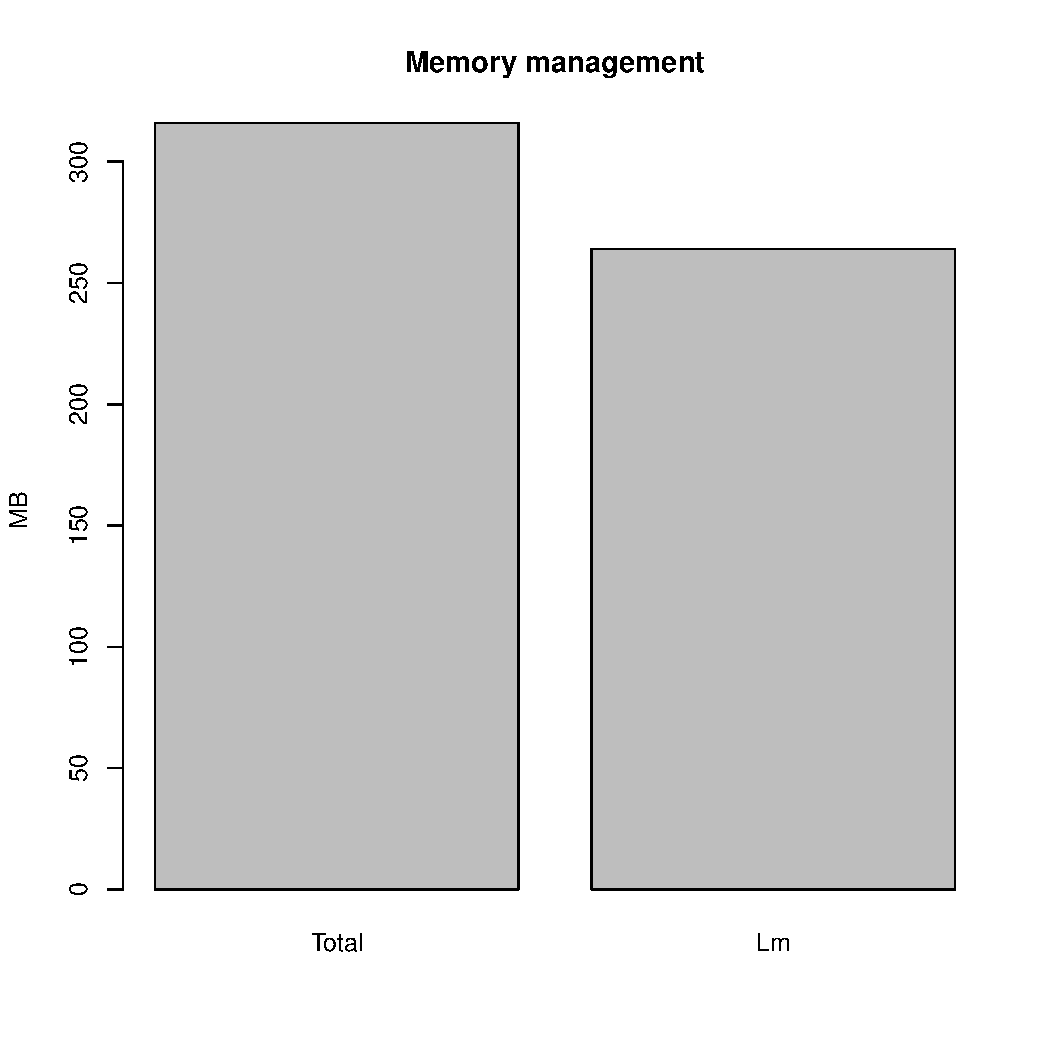
\includegraphics[width=\maxwidth]{figure/unnamed-chunk-20-1} 

\end{knitrout}

\noindent
Then, I write the lm function again for our specific problem; basically I remove useless statements. Then, by storing the memory use of each operation, I plot the result with barplot.
\begin{knitrout}
\definecolor{shadecolor}{rgb}{0.969, 0.969, 0.969}\color{fgcolor}\begin{kframe}
\begin{alltt}
\hlcom{# Size of observations}
\hlstd{obs_size}\hlkwb{=}\hlkwd{object.size}\hlstd{(df}\hlopt{$}\hlstd{y)}\hlopt{/}\hlnum{1e6}
\hlcom{# Lm function for our special case}
\hlstd{lm2} \hlkwb{=} \hlkwa{function} \hlstd{(}\hlkwc{formula}\hlstd{,} \hlkwc{data}\hlstd{)}
\hlstd{\{}
  \hlcom{# Create a new variable which store values of memory used}
  \hlstd{mem_management}\hlkwb{=}\hlkwd{rep}\hlstd{(}\hlnum{0}\hlstd{,}\hlnum{9}\hlstd{)}
  \hlstd{mem_names}\hlkwb{=}\hlkwd{c}\hlstd{(}\hlstr{"cl"}\hlstd{,}\hlstr{"mf"}\hlstd{,}\hlstr{"m"}\hlstd{,}\hlstr{"mf2"}\hlstd{,}\hlstr{"mf3"}\hlstd{,}\hlstr{"mf4"}\hlstd{,}\hlstr{"mt"}\hlstd{,}\hlstr{"y"}\hlstd{,}\hlstr{"x"}\hlstd{)}
  \hlcom{# Total memory used before storing the variables}
  \hlstd{t_m}\hlkwb{=}\hlkwd{mem_used}\hlstd{()}
  \hlcom{# Local variables}
  \hlcom{# 1 : cl}
  \hlstd{cl} \hlkwb{<-} \hlkwd{match.call}\hlstd{()}
  \hlstd{mem_management[}\hlnum{1}\hlstd{]}\hlkwb{=}\hlkwd{mem_used}\hlstd{()}\hlopt{-}\hlstd{t_m}
  \hlstd{t_m}\hlkwb{=}\hlkwd{mem_used}\hlstd{()}
  \hlcom{# 2 : mf1}
  \hlstd{mf} \hlkwb{<-} \hlkwd{match.call}\hlstd{(}\hlkwc{expand.dots} \hlstd{=} \hlnum{FALSE}\hlstd{)}
  \hlstd{mem_management[}\hlnum{2}\hlstd{]}\hlkwb{=}\hlkwd{mem_used}\hlstd{()}\hlopt{-}\hlstd{t_m}
  \hlstd{t_m}\hlkwb{=}\hlkwd{mem_used}\hlstd{()}
  \hlcom{# 3 : m}
  \hlstd{m} \hlkwb{<-} \hlkwd{match}\hlstd{(}\hlkwd{c}\hlstd{(}\hlstr{"formula"}\hlstd{,} \hlstr{"data"}\hlstd{),} \hlkwd{names}\hlstd{(mf),} \hlnum{0L}\hlstd{)}
  \hlstd{mem_management[}\hlnum{3}\hlstd{]}\hlkwb{=}\hlkwd{mem_used}\hlstd{()}\hlopt{-}\hlstd{t_m}
  \hlstd{t_m}\hlkwb{=}\hlkwd{mem_used}\hlstd{()}
  \hlcom{# 4 : mf2}
  \hlstd{mf} \hlkwb{<-} \hlstd{mf[}\hlkwd{c}\hlstd{(}\hlnum{1L}\hlstd{, m)]}
  \hlstd{mem_management[}\hlnum{4}\hlstd{]}\hlkwb{=}\hlkwd{mem_used}\hlstd{()}\hlopt{-}\hlstd{t_m}
  \hlstd{t_m}\hlkwb{=}\hlkwd{mem_used}\hlstd{()}
  \hlcom{# 5 : mf3}
  \hlstd{mf[[}\hlnum{1L}\hlstd{]]} \hlkwb{<-} \hlkwd{quote}\hlstd{(stats}\hlopt{::}\hlstd{model.frame)}
  \hlstd{mem_management[}\hlnum{5}\hlstd{]}\hlkwb{=}\hlkwd{mem_used}\hlstd{()}\hlopt{-}\hlstd{t_m}
  \hlstd{t_m}\hlkwb{=}\hlkwd{mem_used}\hlstd{()}
  \hlcom{# 6 : mf4}
  \hlstd{mf} \hlkwb{<-} \hlkwd{eval}\hlstd{(mf,} \hlkwd{parent.frame}\hlstd{())}
  \hlstd{mem_management[}\hlnum{6}\hlstd{]}\hlkwb{=}\hlkwd{mem_used}\hlstd{()}\hlopt{-}\hlstd{t_m}
  \hlstd{t_m}\hlkwb{=}\hlkwd{mem_used}\hlstd{()}
  \hlcom{# 7 : mt}
  \hlstd{mt} \hlkwb{<-} \hlkwd{attr}\hlstd{(mf,} \hlstr{"terms"}\hlstd{)}
  \hlstd{mem_management[}\hlnum{7}\hlstd{]}\hlkwb{=}\hlkwd{mem_used}\hlstd{()}\hlopt{-}\hlstd{t_m}
  \hlstd{t_m}\hlkwb{=}\hlkwd{mem_used}\hlstd{()}
  \hlcom{# 8 : y}
  \hlstd{y} \hlkwb{<-} \hlkwd{model.response}\hlstd{(mf,} \hlstr{"numeric"}\hlstd{)}
  \hlstd{mem_management[}\hlnum{8}\hlstd{]}\hlkwb{=}\hlkwd{mem_used}\hlstd{()}\hlopt{-}\hlstd{t_m}
  \hlstd{t_m}\hlkwb{=}\hlkwd{mem_used}\hlstd{()}
  \hlcom{# 9 : x}
  \hlstd{x} \hlkwb{<-} \hlkwd{model.matrix}\hlstd{(mt, mf)}
  \hlstd{mem_management[}\hlnum{9}\hlstd{]}\hlkwb{=}\hlkwd{mem_used}\hlstd{()}\hlopt{-}\hlstd{t_m}
  \hlstd{t_m}\hlkwb{=}\hlkwd{mem_used}\hlstd{()}
  \hlcom{# Plot memory management}
  \hlkwd{barplot}\hlstd{(mem_management}\hlopt{/}\hlnum{1e6}\hlstd{,}\hlkwc{names.arg} \hlstd{= mem_names,}\hlkwc{ylab}\hlstd{=}\hlstr{"MB"}\hlstd{,}
          \hlkwc{main}\hlstd{=}\hlstr{"Memory management"}\hlstd{)}
  \hlkwd{lines}\hlstd{(}\hlkwc{x}\hlstd{=}\hlnum{0}\hlopt{:}\hlnum{11}\hlstd{,}\hlkwc{y}\hlstd{=}\hlkwd{rep}\hlstd{(obs_size,}\hlnum{12}\hlstd{))}
  \hlkwd{text}\hlstd{(}\hlkwc{x}\hlstd{=}\hlnum{3}\hlstd{,}\hlkwc{y}\hlstd{=obs_size}\hlopt{+}\hlnum{.5} \hlstd{,}\hlkwc{labels} \hlstd{=} \hlkwd{c}\hlstd{(}\hlstr{"size of observations"}\hlstd{))}

  \hlcom{# lm.fit call}
  \hlstd{z} \hlkwb{<-} \hlkwd{lm.fit}\hlstd{(x, y,} \hlkwc{singular.ok} \hlstd{=} \hlnum{TRUE}\hlstd{)}
  \hlkwd{class}\hlstd{(z)} \hlkwb{<-} \hlkwd{c}\hlstd{(}\hlkwa{if} \hlstd{(}\hlkwd{is.matrix}\hlstd{(y))} \hlstr{"mlm"}\hlstd{,} \hlstr{"lm"}\hlstd{)}
  \hlstd{z}\hlopt{$}\hlstd{xlevels} \hlkwb{<-} \hlkwd{.getXlevels}\hlstd{(mt, mf)}
  \hlstd{z}\hlopt{$}\hlstd{call} \hlkwb{<-} \hlstd{cl}
  \hlstd{z}\hlopt{$}\hlstd{terms} \hlkwb{<-} \hlstd{mt}
  \hlstd{z}\hlopt{$}\hlstd{model} \hlkwb{<-} \hlstd{mf}
  \hlkwd{list}\hlstd{(z,mem_management)}
\hlstd{\}}
\hlkwd{lm2}\hlstd{(y}\hlopt{~}\hlstd{.,}\hlkwc{data} \hlstd{= df)}
\end{alltt}
\end{kframe}
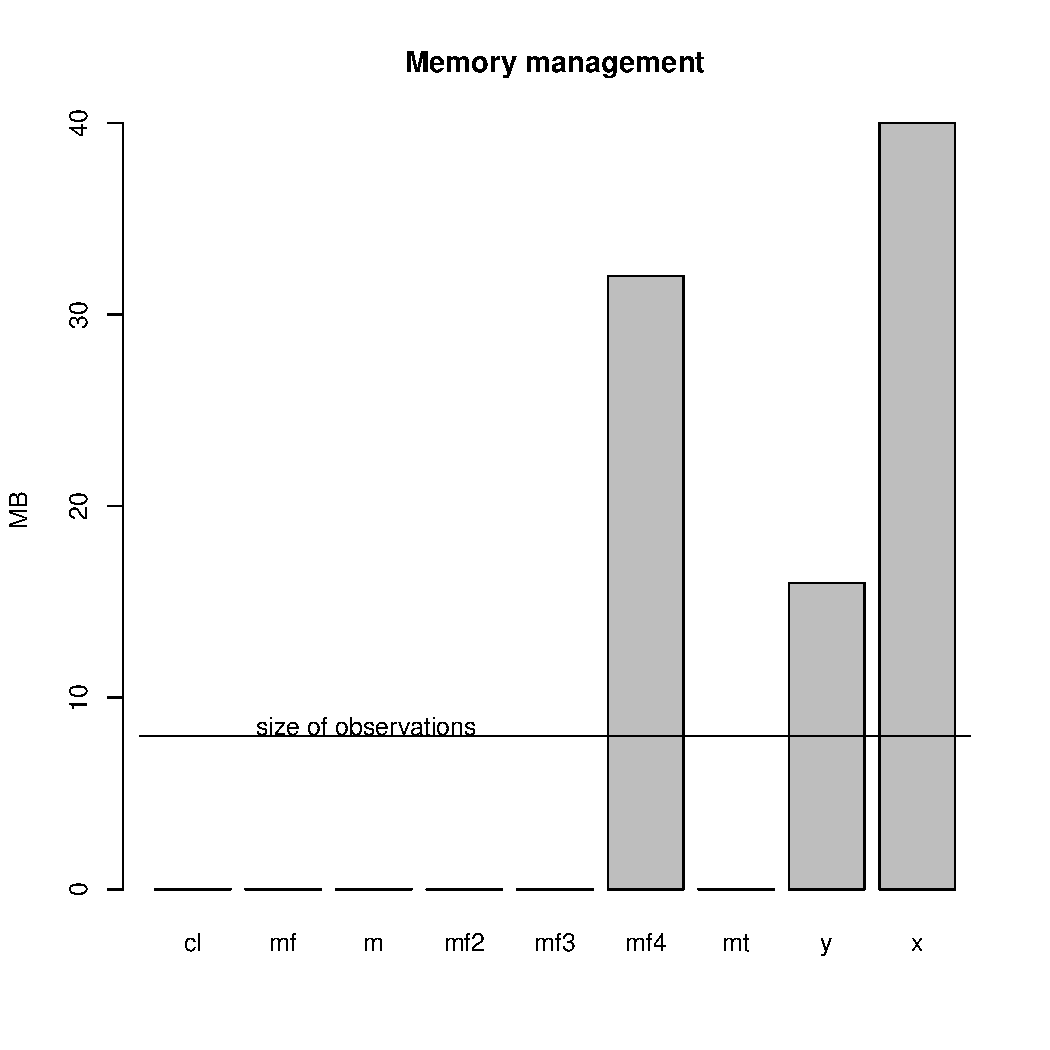
\includegraphics[width=\maxwidth]{figure/unnamed-chunk-21-1} 
\begin{kframe}\begin{lstlisting}[basicstyle=\ttfamily,breaklines=true]
## [[1]]
## 
## Call:
## lm2(formula = y ~ ., data = df)
## 
## Coefficients:
## (Intercept)           x1           x2           x3  
##   0.0021041    0.0011744   -0.0048279   -0.0002561  
## 
## 
## [[2]]
## [1]     -416      392      232        0      112 32003112
## [7]      112 16000280 40000688
\end{lstlisting}
\end{kframe}
\end{knitrout}
\noindent
If figure out how much total memory is in use in lm() at the point at which lm.fit() is called and I compare the additional memory use to the memory used in the global environment to store the observations and covariates. The latter is given by the sum of the second attribute of lm2 function.
\begin{knitrout}
\definecolor{shadecolor}{rgb}{0.969, 0.969, 0.969}\color{fgcolor}\begin{kframe}
\begin{alltt}
\hlkwd{barplot}\hlstd{(}\hlkwd{c}\hlstd{(}\hlkwd{object.size}\hlstd{(df}\hlopt{$}\hlstd{y),}\hlkwd{sum}\hlstd{(}\hlkwd{lm2}\hlstd{(y}\hlopt{~}\hlstd{.,}\hlkwc{data} \hlstd{= df)[[}\hlnum{2}\hlstd{]]))}\hlopt{/}\hlnum{1e6}\hlstd{,}
        \hlkwc{names.arg} \hlstd{=} \hlkwd{c}\hlstd{(}\hlstr{"Variables"}\hlstd{,}\hlstr{"Total before lm.fit()"}\hlstd{),}
        \hlkwc{ylab}\hlstd{=}\hlstr{"MB"}\hlstd{,}\hlkwc{main}\hlstd{=}\hlstr{"Memory management"}\hlstd{)}
\end{alltt}
\end{kframe}
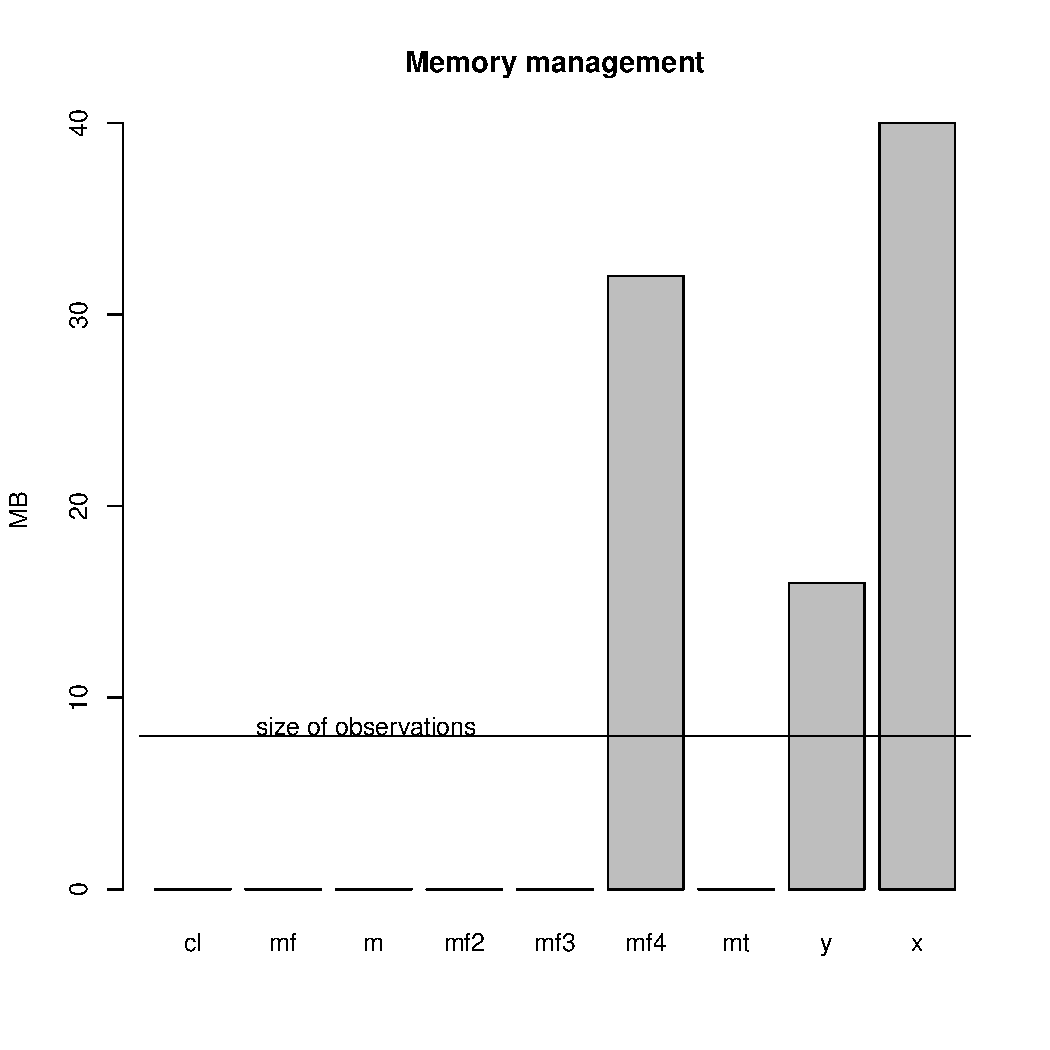
\includegraphics[width=\maxwidth]{figure/unnamed-chunk-22-1} 

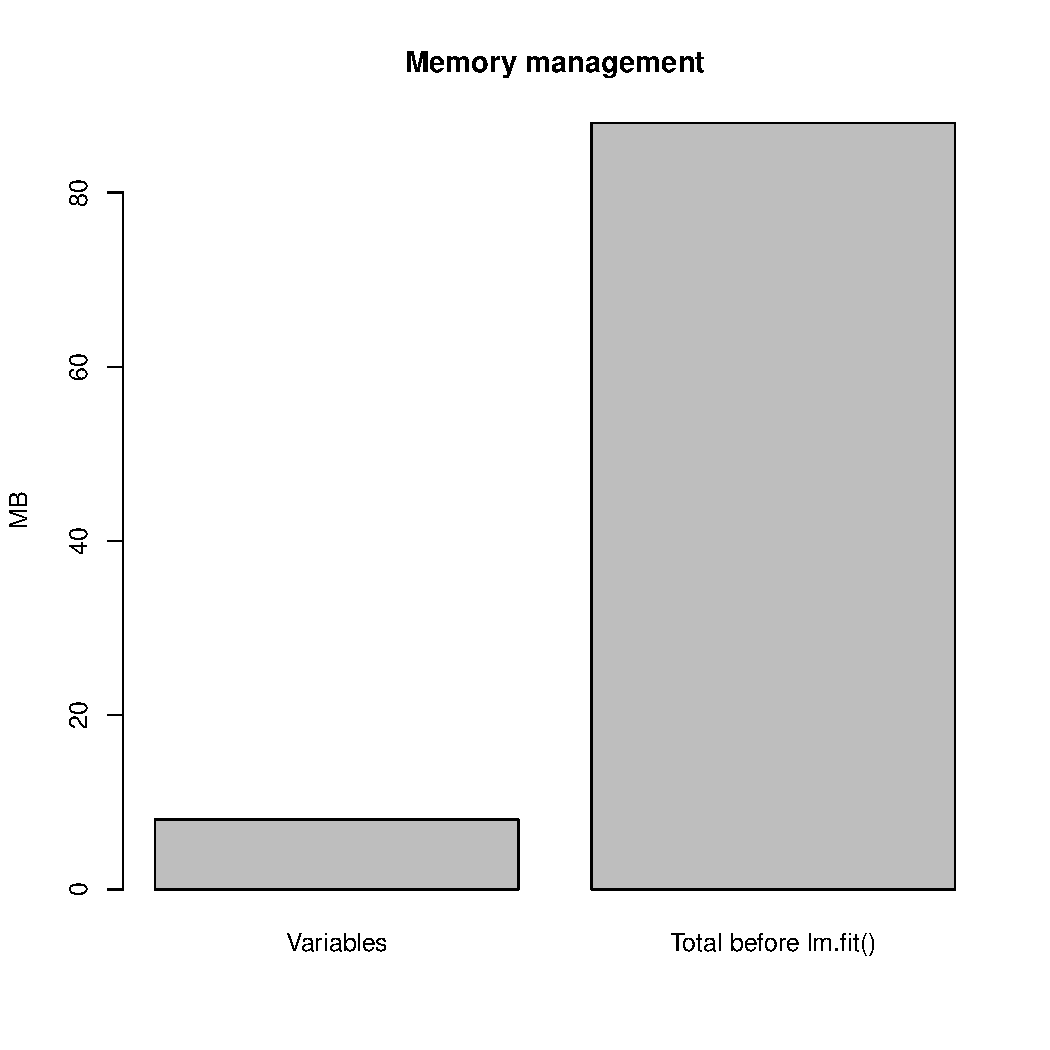
\includegraphics[width=\maxwidth]{figure/unnamed-chunk-22-2} 

\end{knitrout}
\noindent
An explanation of why some of the vectors and matrices are larger than 8 bytes per number, is that extra memory is used to store compute other variables such as the residuals and the fitted values. \\
To optimize memory used, we can directly compute the result of the least square estimate:
\begin{knitrout}
\definecolor{shadecolor}{rgb}{0.969, 0.969, 0.969}\color{fgcolor}\begin{kframe}
\begin{alltt}
\hlstd{x}\hlkwb{=}\hlkwd{as.matrix}\hlstd{(df[,}\hlnum{2}\hlopt{:}\hlnum{4}\hlstd{])}
\hlstd{y}\hlkwb{=}\hlkwd{as.matrix}\hlstd{(df[,}\hlnum{1}\hlstd{])}
\hlstd{t_m}\hlkwb{=}\hlkwd{mem_used}\hlstd{()}
\hlstd{Beta} \hlkwb{=} \hlkwd{solve}\hlstd{(}\hlkwd{crossprod}\hlstd{(x,x),} \hlkwd{crossprod}\hlstd{(x,y))}
\hlstd{beta_mem}\hlkwb{=}\hlkwd{mem_used}\hlstd{()}\hlopt{-}\hlstd{t_m}
\hlcom{# New value}
\hlstd{beta_mem}
\end{alltt}
\begin{lstlisting}[basicstyle=\ttfamily,breaklines=true]
## 16.3 kB
\end{lstlisting}
\begin{alltt}
\hlcom{# Plot}
\hlkwd{barplot}\hlstd{(}\hlkwd{c}\hlstd{(}\hlkwd{object.size}\hlstd{(df}\hlopt{$}\hlstd{y),}\hlkwd{sum}\hlstd{(}\hlkwd{lm2}\hlstd{(y}\hlopt{~}\hlstd{.,}\hlkwc{data} \hlstd{= df)[[}\hlnum{2}\hlstd{]]),beta_mem)}\hlopt{/}\hlnum{1e6}\hlstd{,}
        \hlkwc{names.arg} \hlstd{=} \hlkwd{c}\hlstd{(}\hlstr{"Variables"}\hlstd{,}\hlstr{"Total before lm.fit()"}\hlstd{,}\hlstr{"Using Beta"}\hlstd{),}
        \hlkwc{ylab}\hlstd{=}\hlstr{"MB"}\hlstd{,}\hlkwc{main}\hlstd{=}\hlstr{"Memory management"}\hlstd{)}
\end{alltt}
\end{kframe}
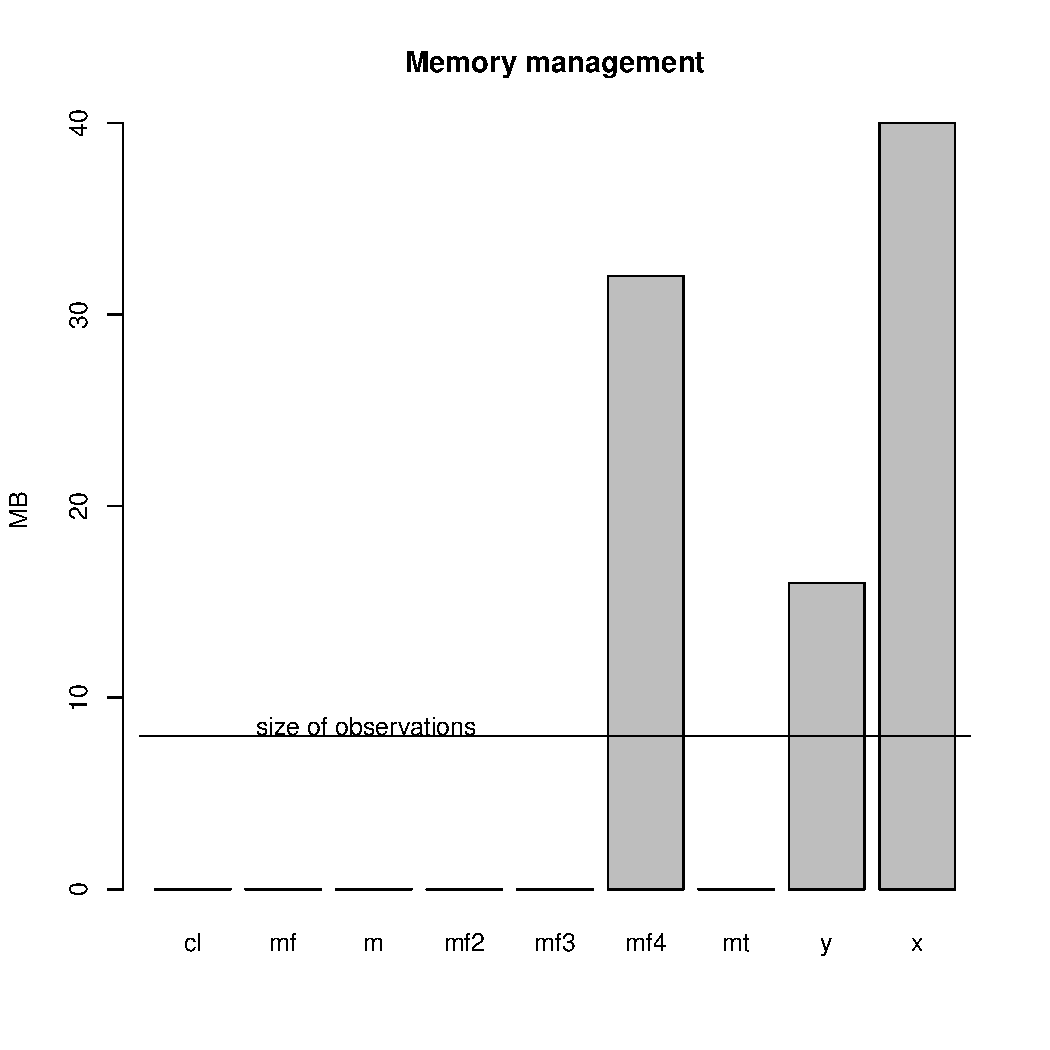
\includegraphics[width=\maxwidth]{figure/unnamed-chunk-23-1} 

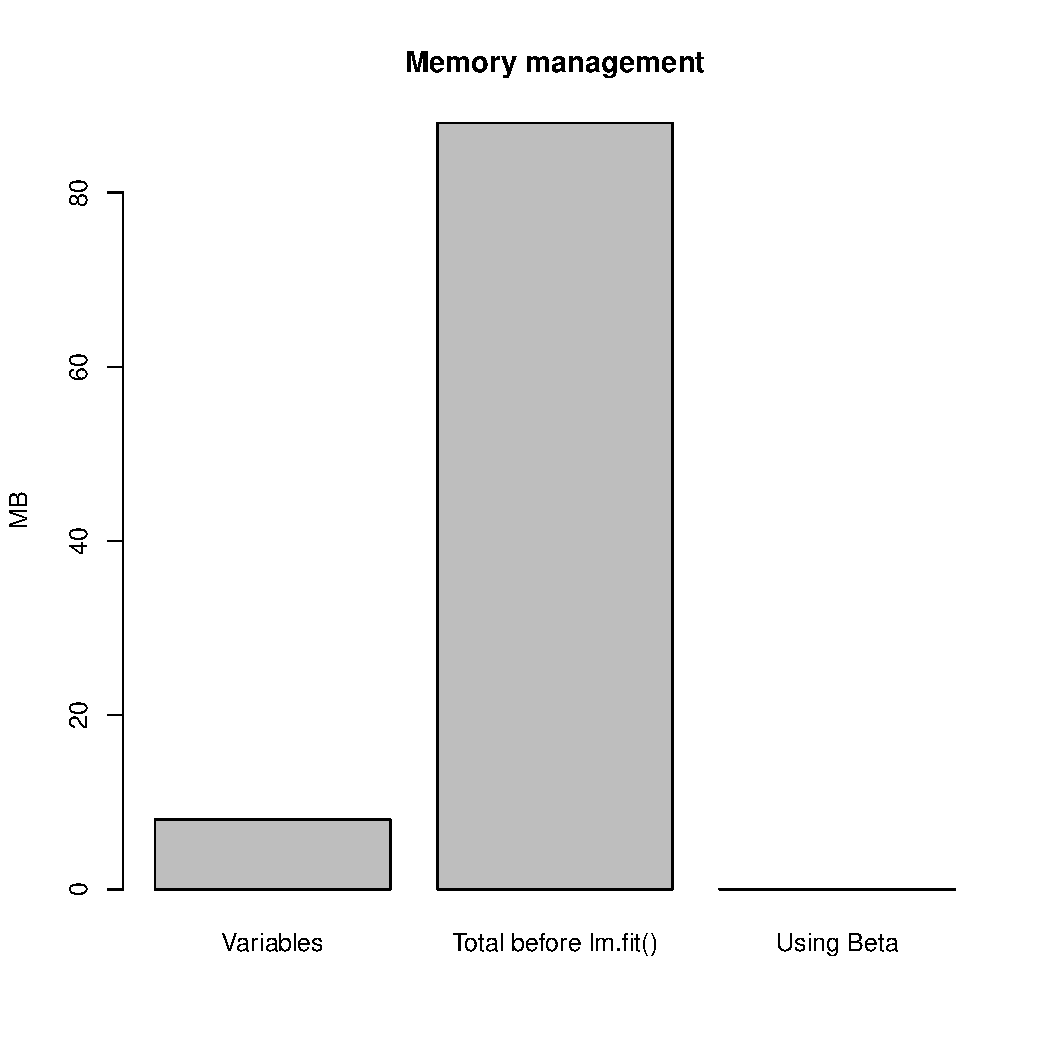
\includegraphics[width=\maxwidth]{figure/unnamed-chunk-23-2} 

\end{knitrout}
\noindent
Now, we see that the memory used to store Beta is almost nothing compared to the data used to compute lm(). However, by doing this, we do not have directly access to relevant information such as residuals or the fitted values. We can see that the results are very close to each other:
\begin{knitrout}
\definecolor{shadecolor}{rgb}{0.969, 0.969, 0.969}\color{fgcolor}\begin{kframe}
\begin{alltt}
\hlcom{# Using lm2}
\hlkwd{lm2}\hlstd{(y}\hlopt{~}\hlstd{.,}\hlkwc{data} \hlstd{= df)[[}\hlnum{1}\hlstd{]]}\hlopt{$}\hlstd{coefficients[}\hlnum{2}\hlopt{:}\hlnum{4}\hlstd{]}
\end{alltt}
\end{kframe}
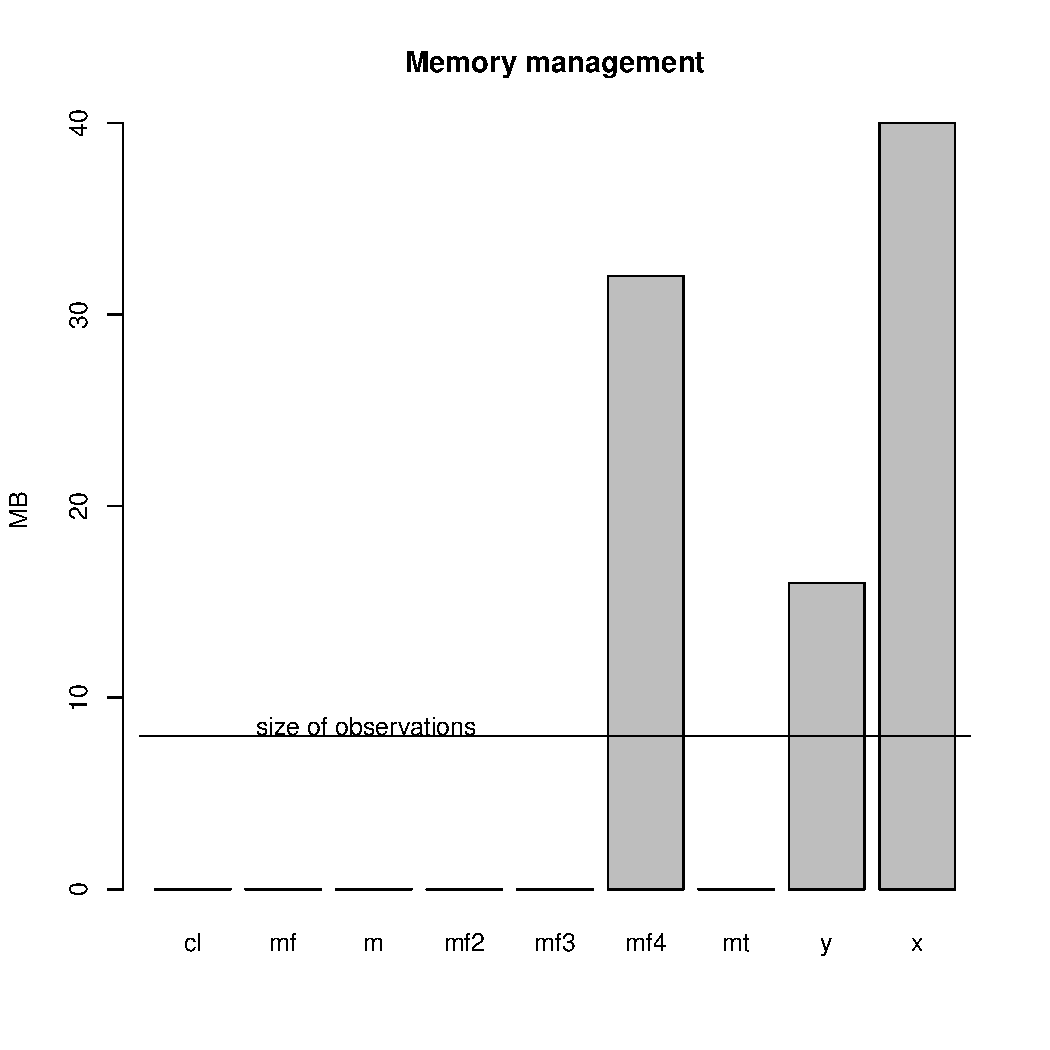
\includegraphics[width=\maxwidth]{figure/unnamed-chunk-24-1} 
\begin{kframe}\begin{lstlisting}[basicstyle=\ttfamily,breaklines=true]
##            x1            x2            x3 
##  0.0011743658 -0.0048279397 -0.0002560523
\end{lstlisting}
\begin{alltt}
\hlcom{# Using LSE Beta}
\hlkwd{t}\hlstd{(Beta)}
\end{alltt}
\begin{lstlisting}[basicstyle=\ttfamily,breaklines=true]
##              x1           x2            x3
## [1,] 0.00135383 -0.003337436 -0.0002712319
\end{lstlisting}
\end{kframe}
\end{knitrout}

\end{document}
